Figure \ref{fig:gantt_chart} portrays a Gantt chart outlining the approach from the section above. At the end of each week, I will evaluate this schedule to update the chart with any progress changes. I intend to approach this schedule as a `live' document with constant change by preserving a complete version history.

\begin{figure}[h]
    \centering
    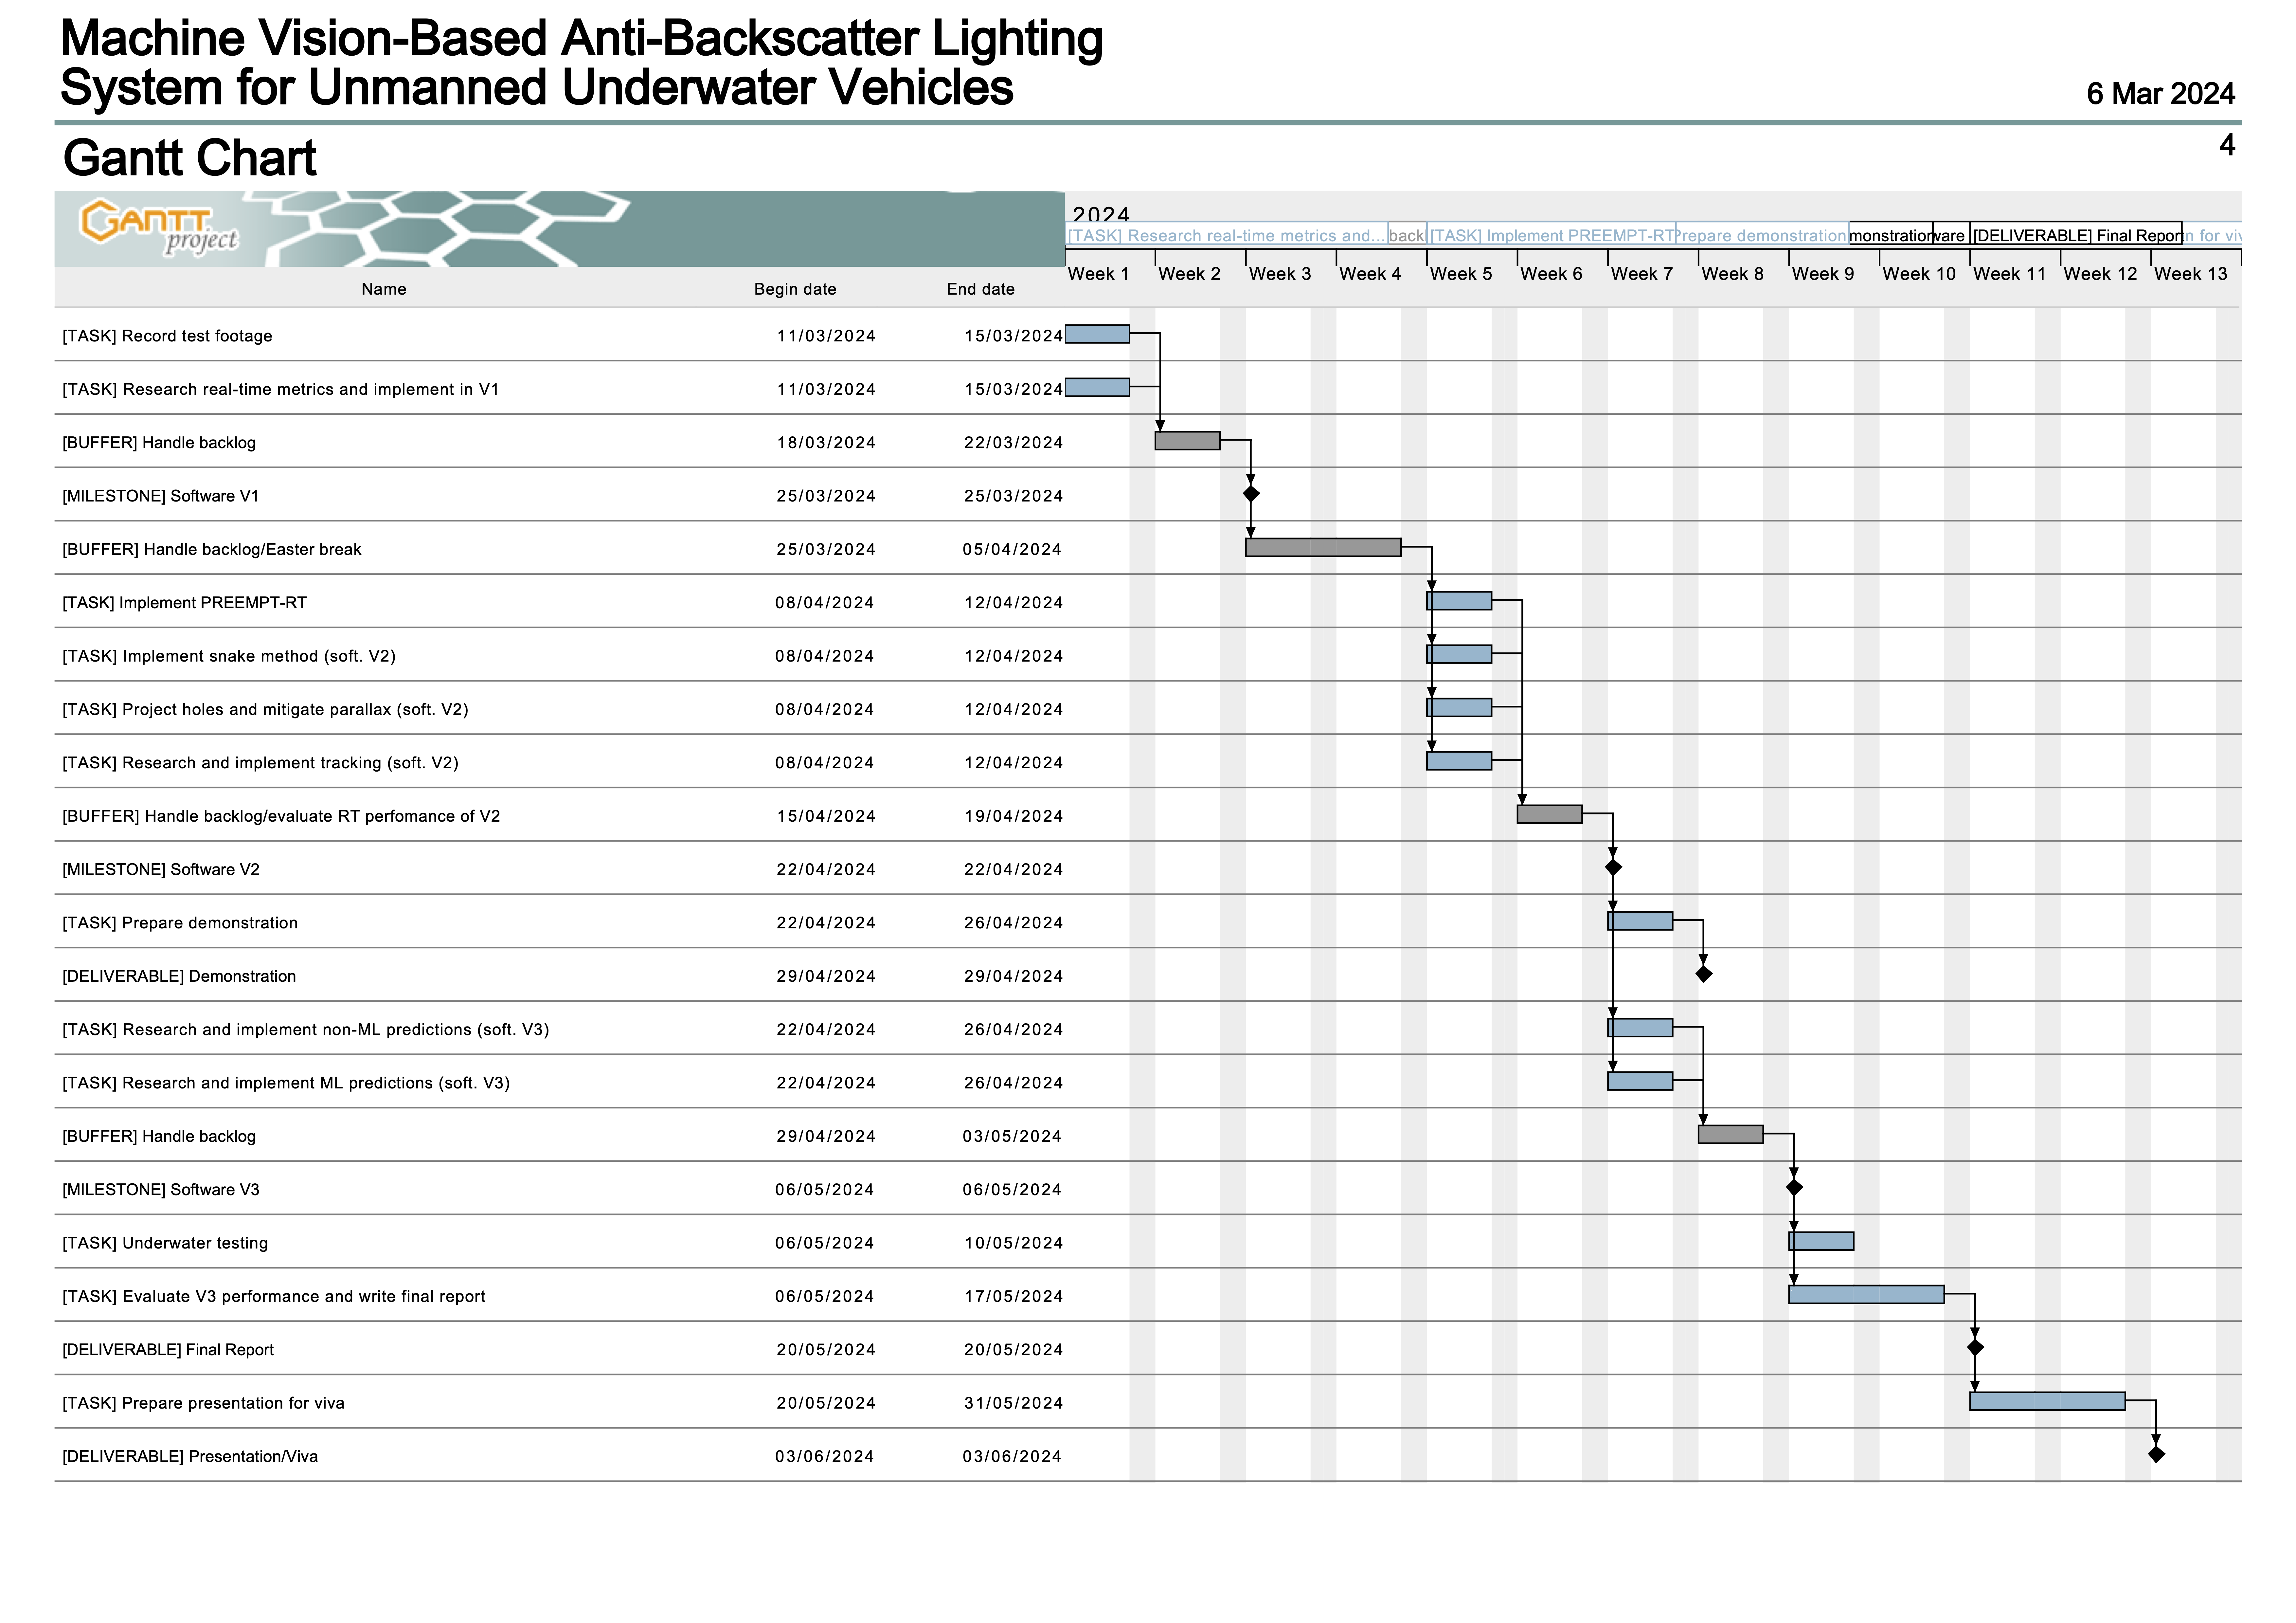
\includegraphics[width=0.89\textwidth]{assets/gantt_chart.png}
    \caption{A Gantt chart illustrating the overall project schedule plan.}
    \label{fig:gantt_chart}
\end{figure}

This report has described the current progress status, outlining the ultimate goal, the aims, and an investigation of background information which has decided some project choices. The report has also discussed the plan for the remaining tasks, illustrated with a detailed and active Gantt chart schedule. The information this report details is a sufficient starting point for experimental work to enable additional research as the development of this system continues.
